\documentclass[conference]{IEEEtran}

% 図表用の最小パッケージ(本文から独立)
\usepackage{graphicx}
\usepackage{tikz}
\usepackage{pgfplots}
\pgfplotsset{compat=1.18}
\usetikzlibrary{arrows.meta,positioning}

\begin{document}
\title{Figures and Tables for ``FeFET CMOS 0.18~$\mu$m Integration Study''}
\author{}
\maketitle

\section*{Figures and Tables}

% -------- Fig.1(フロー図:あなたの最新版TikZをここへ) --------
\begin{figure}[!t]\centering
% \begin{tikzpicture}[...] ... \end{tikzpicture}
\caption{Placement of the FeFET gate-last module within the 0.18~$\mu$m CMOS baseline (vertical layout).}
\end{figure}

% -------- Table I(追加マスク) --------
\begin{table}[!t]\centering
\caption{Added masks / process steps relative to baseline logic.}
\begin{tabular}{|c|c|l|}\hline
Step & Mask & Comment\\ \hline
FE metal gate & +1 & Reuse analog option route\\
FE anneal & 0 & Performed in BEOL furnace (no extra mask)\\ \hline
\end{tabular}
\end{table}

% -------- Fig.2(Endurance:pgfplots) --------
\begin{figure}[!t]\centering
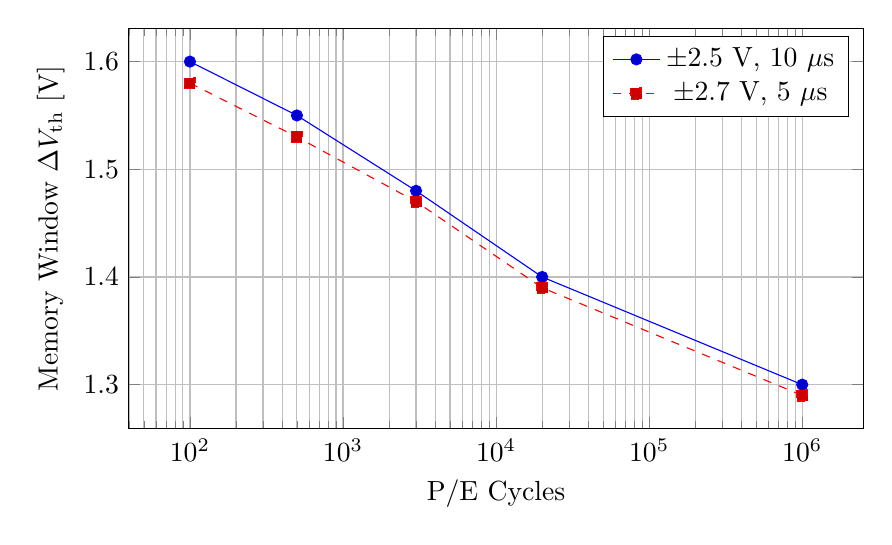
\begin{tikzpicture}
\begin{axis}[
  width=0.9\linewidth,height=0.55\linewidth,
  xlabel={P/E Cycles}, xmode=log, log basis x=10,
  ylabel={Memory Window $\Delta V_{\mathrm{th}}$ [V]},
  grid=both]
\addplot+[mark=*] coordinates {(1e2,1.6) (5e2,1.55) (3e3,1.48) (2e4,1.40) (1e6,1.30)};
\addlegendentry{$\pm 2.5$ V, 10 $\mu$s}
\addplot+[mark=square*, dashed] coordinates {(1e2,1.58) (5e2,1.53) (3e3,1.47) (2e4,1.39) (1e6,1.29)};
\addlegendentry{$\pm 2.7$ V, 5 $\mu$s}
\end{axis}
\end{tikzpicture}
\caption{Schematic endurance behavior of HZO-FeFETs in a 0.18~$\mu$m flow.}
\end{figure}

% -------- Fig.3(Wake-up と Retention:縦並び) --------
\begin{figure}[!t]\centering
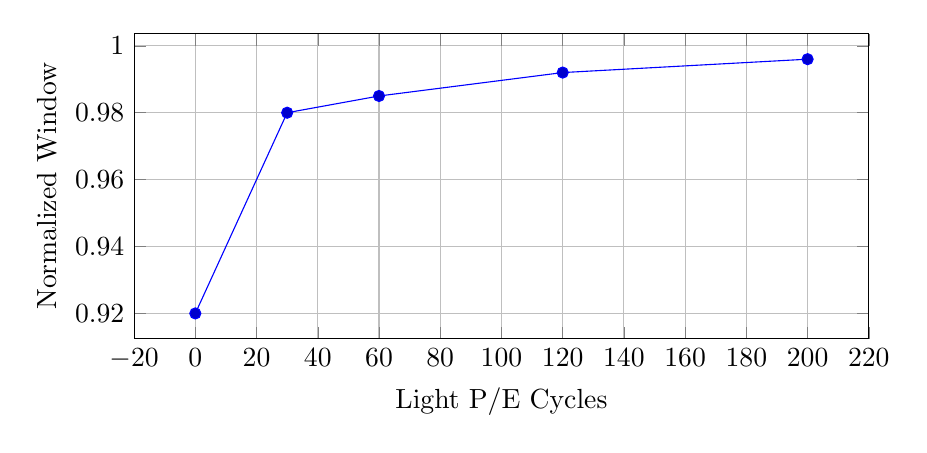
\begin{tikzpicture}
\begin{axis}[
  width=0.9\linewidth,height=0.45\linewidth,
  xlabel={Light P/E Cycles}, ylabel={Normalized Window}, grid=both]
\addplot+[mark=*] coordinates {(0,0.92) (30,0.98) (60,0.985) (120,0.992) (200,0.996)};
\end{axis}
\end{tikzpicture}

\vspace{0.6em}

\begin{tikzpicture}
\begin{axis}[
  width=0.9\linewidth,height=0.45\linewidth,
  xmode=log, log basis x=10, grid=both,
  xlabel={Time $t$ @ 85$^\circ$C (s)}, ylabel{$\Delta V_{\mathrm{th}}(t)/\Delta V_{\mathrm{th}}(t_0)$}]
\addplot+[mark=*] coordinates {(1e2,0.995) (1e3,0.985) (1e4,0.972) (1e5,0.960) (1e6,0.950)};
\end{axis}
\end{tikzpicture}
\caption{Wake-up (top) and retention projection at 85$^\circ$C (bottom).}
\end{figure}

% -------- Fig.4(TDDB Weibull) --------
\begin{figure}[!t]\centering
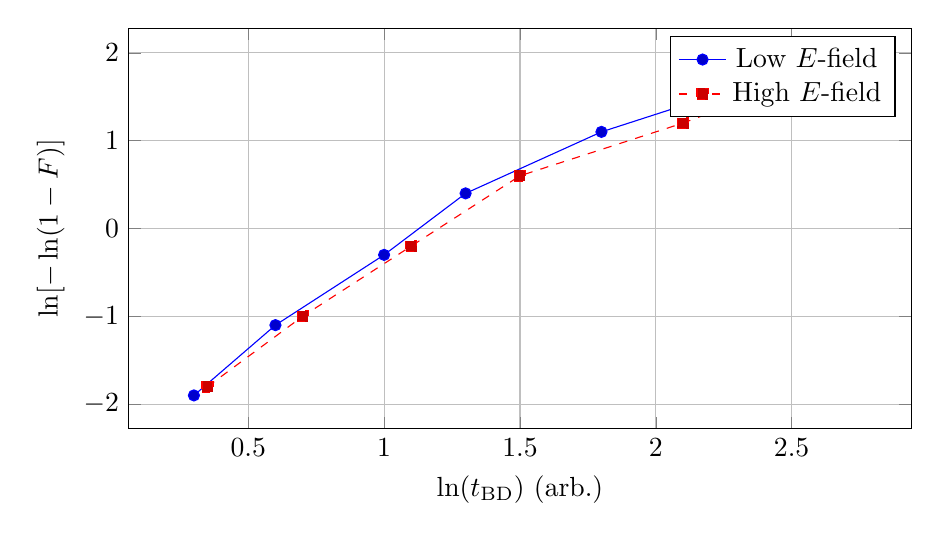
\begin{tikzpicture}
\begin{axis}[
  width=0.95\linewidth,height=0.55\linewidth,
  xlabel={$\ln(t_{\mathrm{BD}})$ (arb.)},
  ylabel={$\ln[-\ln(1-F)]$}, grid=both]
\addplot+[mark=*] coordinates {(0.3,-1.9) (0.6,-1.1) (1.0,-0.3) (1.3,0.4) (1.8,1.1) (2.3,1.6)};
\addlegendentry{Low $E$-field}
\addplot+[mark=square*, dashed] coordinates {(0.35,-1.8) (0.7,-1.0) (1.1,-0.2) (1.5,0.6) (2.1,1.2) (2.7,1.9)};
\addlegendentry{High $E$-field}
\end{axis}
\end{tikzpicture}
\caption{TDDB Weibull representation at two stress fields (illustrative).}
\end{figure}

\end{document}
